\chapter{Equazione del calore e metodo Perona-Malik}
L'equazione del calore, come facilmente intuibile, è stata formulata per determinare l'evoluzione di un sistema isolato che presenta al suo interno una data distribuzione di calore.\\
Euristicamente, non è difficile pensare che si possano codificare (pensando ad un'immagine in bianco e nero) i pixel più luminosi come punti "più caldi", mentre quelli più scuri come punti "più freddi" ed applicare così l'equazione del calore all'immagine.\\
Mediante uno script MATLAB si può dunque osservare come quest'ultima operi nella pratica, sfruttando una approssimazione alle \textbf{differenze finite } utile per il calcolo delle derivate.\\
\section{Metodo delle differenze finite}
Il metodo delle differenze finite, come anticipato, viene impiegato nel calcolo approssimato delle derivate. Il procedimento segue dalla definizione in sè di derivata. \\La scelta adottata per la suddetta approssimazione risulterà dunque essere:\\
\vspace{2em}
\centering 
{\Large$\frac{du}{dx} \approx \frac{u_{i+1} - u_i}{\Delta(x)} $.}\\
~\\
~\\
~\\
~\\
~\\
~\\
~\\
~\\
~\\
~\\
~\\
~\\

\newpage
\raggedright
In particolare, dal momento che la derivata seconda coincide con la derivata della derivata prima, allora quest'ultima può essere approssimata nel seguente modo:\\
\centering    
{\large
\begin{align*}
\frac{d^2u}{dx^2} \approx &
\frac{
(\frac{u_{i+1} - u_i}{\Delta(x)})_{i+1} 
- 
(\frac{u_{i+1} - u_i}{\Delta(x)})_i
}{\Delta(x)}
\\
\vline
\\
= &
\frac{
\frac{(u_{i+1} - u_i)_{i+1}}{\Delta(x)} 
-   
\frac{(u_{i+1} - u_i)_i}{\Delta(x)}
}{\Delta(x)}
\\
\vline 
\\
= &
\frac{
\frac{(u_{i+2} - u_{i+1})}{\Delta(x)} 
- 
\frac{(u_{i+1} - u_i)}{\Delta(x)}
}{\Delta(x)}
\\
\vline 
\\
= &
\frac{
\frac{(u_{i+2} - u_{i+1}) 
- 
(u_{i+1} - u_i)}{\Delta(x)}
}{\Delta(x)}
\\
\vline
\\
= &
\frac{
(u_{i+2} - u_{i+1}) 
- 
(u_{i+1} - u_i)}
{\Delta(x)^2}
\\
\vline 
\\
= &
\frac{
 u_{i+2} - u_{i+1} 
-u_{i+1} + {u_i}}
{\Delta(x)^2}
.\\
\end{align*}
}
\raggedright
Per una ottenere una stima accurata, è bene utilizzare un valore di $\Delta(x)$ quanto più basso possibile. La migliore è guardare la differenza tra un pixel e quello adiacente ossia $\Delta(x)=1$, ma allora 
{\large
$$\frac{d^2u}{dx^2} \approx
\frac{
 u_{i+2} - u_{i+1} 
-u_{i+1} + u_i}
{\Delta(x)^2} = u_{i+2} -2 u_{i+1} + u_i.$$
}
\`E chiaro che scorrendo tutti gli indici questo è equivalente a $u_{i+1} -2 u_i + u_{i-1}.$

In sintesi si può utilizzare per il calcolo del laplaciamo l'approssimazione \\
\vspace{2pt}
\centering 
{\Large
$\frac{d^2u}{dx^2} \approx u_{i+1} -2 u_i + u_{i-1}$.\\
}
\vspace{2pt}
\raggedright
\newpage
\subsection{Errore di troncamento}

Vale la pena di fare qualche considerazione sull'errore di troncamento che si commette adottando queste approssimazioni.\\
Per definizione, l'errore è la differenza tra il valore esatto e quello approssimato, ossia: 

$$
\frac{d^2u}{dx^2}\vline_{x_i}-\frac{u_{i+1}-u_i}{\Delta(x)}\approx \frac{\Delta(x)^2}{2} \frac{d^2u}{dx^2}\vline_\xi.
$$

Risulta quindi evidente che l'errore dipende da $\Delta(x)^2$. 
Ad un'attenta analisi possiamo vedere che tra i metodi di approssimazione in avanti, in indietro o centrale, il calcolo dell'errore portato dai primi due sono uguali tra di loro, quello centrale invece è diverso, esso dipende da un $\Delta(x)^3$ e non da un $\Delta(x)^2$, questo vuol dire che per $\Delta(x)<1$ funziona meglio, per $\Delta(x)>1$ funziona peggio. Nel caso in analisi $\Delta(x)=1$ quindi la scelta è indifferente.
%Ma procediamo con ordine.\\

Per brevità di notazione poniamo $\Delta(x)=h$.\\
Dagli sviluppi di Taylor in $x_j$ di
$u(x_{j \pm 1}) = u(x_j \pm h)$ fino al terzo ordine, si ottiene che

$$
u''(x_j) =\frac{u(x_{j+1}) - 2u(x_j) + u(x_{j-1})}{h^2} -\frac{1}{12} u^{(4)}(\xi_j)h^2
$$

dove $\xi_j$ e un punto opportuno in $(x_{j-1} , x{j+1})$. Quindi, considerando il problema modello con condizoni di Dirichlet, per $j = 1,...,N-1$, si può scrivere che

$$
\frac{-u(x_{j+1}) + 2u(x_j) -u(x{j-1})}{h^2}
 + \frac{1}{12} u^{(4)}(\xi_j)h^2 + \sigma(x_j)u(x_j) = f(x_j) .
$$

Introducendo la notazione $\tau_{j}=\frac{1}{12} u(4)(\xi_j)h^2$ (errore di troncamento locale) e ponendo:\\

$\boldsymbol{u}=[u_x...u_{N-1}]^T$\\
$\boldsymbol{\tau_h}=[\tau_x...\tau_{N-1}]^T$\\
$\boldsymbol{b_h}=[(f(x_1) + \frac{g_0}{h^2},f(x_2),...,f(x_{N-2}),f(x_{N-1}) + \frac{g_1}{h^2}]^T$\\

si può allora scrivere in forma matriciale,
$A_h\boldsymbol{u} = \boldsymbol{b_h} + \boldsymbol{\tau_h}$
dove $A_h = \frac{1}{h^2}
 tridiag(-1,2,-1) + diag(\sigma_1, ... ,\sigma_{N-1}) e \sigma_j = \sigma(x_j)$.\\
\vspace{1em}
Il metodo alle differenze finite consiste allora nel determinare un’approssimazione $u_h$ di
u andando a risolvere il sistema lineare
$A_h\boldsymbol{u_h} = \boldsymbol{b_h}.$
Osserviamo che $\boldsymbol{u_h}$ risulta ben definito in quanto $A_h$ è una matrice non singolare.\\

\vspace{1em}

Risultando che $\boldsymbol{\tau_h}$ tende a zero quando h tende a zero, il metodo dicesi consistente. In particolare nel caso in analisi, come osservato in partenza, risulta $\boldsymbol{\tau_h} = O(h^2)$ .\\
Tuttavia la consistenza non assicura da sola la convergenza del metodo.\\
Per studiarne laconvergenza è necessario considerare il comportamento dell’errore $\boldsymbol{e_h} = \boldsymbol{u_h} -\boldsymbol{u}$ quando h tende a zero. Dato che risulta $A_h\boldsymbol{e_h} = \boldsymbol{\tau_h}$, e quindi $\boldsymbol{e_h} = A_h^{-1} \boldsymbol{\tau_h}$ si può quindi scrivere: $||\boldsymbol{e_h}||\geq ||A_h^{-1}|| |\boldsymbol{\tau_h}||$\\
Il passaggio successiovo è far vedere che, lavorando in norma infinito, si è in grado di trovare una costante che, per ogni $h$, maggiora $||A_h^{-1}||$. \\ 
\newpage
A questo scopo osservando che si può dimostrare che sia $A_h$ che la matrice $A_{0h} = \frac{1}{h^2} tridiag(-1,2,-1)$ hanno inversa non negativa, e si ha: 

$$A_{0h}^{-1}-A{h}^{-1}=A_{0h}^{-1}(A_h-A_{0h})A_h^{-1}\geq0.$$

Per le ipotesi su $\sigma$ questo implica $A_h^{-1}||\leq A_{0h}^{-1}||$
osserviamo che
$||A_{0h}^{-1}||=max_j(A_{0h}^{-1}\boldsymbol{e})_j$ dove $\boldsymbol{e}$ indica il vettore di tutti 1.\\
Osservando che la soluzione esatta del problema $-u'' = 1, u(0) = u(1) = 0$, è il polinomio di secondo grado $\phi(x) = \frac{x(1-x)}{2}$, si può concludere che $A_{0h}^{-1}\boldsymbol{e})_j=\phi(x_j)$ e quindi che $A_h^{-1}||\leq A_{0h}^{-1}||\leq max_{0<x<1}|\phi_x|$.\\
Questo risultato di stabilità ci permette di concludere che l’errore $\boldsymbol{e_h}$ ha lo stesso ordine dell’errore di troncamento $\boldsymbol{\tau_h}$ e di conseguenza che il metodo è convergente del secondo ordine.
Si noti che l’uniforme limitatezza della norma di $A_h^{-1}$ implica che il metodo numerico sia stabile. 




\newpage

\section{L'equazione del calore}

\raggedright

Il metodo delle differenze finite sarà impiegato in uno script MATLAB per l'implementazione dell'equazione del calore, è bene quindi prenderla in esame.

\begin{equation} 
\begin{cases}

\frac{\partial u}{\partial t}(t,x)-\Delta u(t,x) = 0 \ x \in \mathbb R^2, t\ge 0 \ .\\ 

u(0,x) = u_0(x)\ . \\

\end{cases}
\end{equation}

L'equazione del calore, come anticipato, determina l'evoluzione di un sistema isolato che presenta al suo interno una data distribuzione di calore. \`E banale pensare che con il passare del tempo il calore si distribuisca, tendendo per un tempo infinito ad una distribuzione uniforme.

\vspace{1em}

Applicando l'equazione del calore si ottiene quindi un'immagine sempre più "liscia", di fatto una sfocatura, e per un numero di iterazioni idealmente infinito si giungerebbe ad una distribuzione uniforme di colore, ossia una tinta unita.

\vspace{1em}
%\newpage

Il seguente script MATLAB illustra come questo processo opera nella pratica.

\begin{lstlisting}[language=MATLAB]
Im=imread('parrot.jpeg');   %Apro l'immmagine
Im=rgb2gray(Im);            %La trasformo in bianco e nero
Im = imnoise(Im,'gaussian');%Aggiungo del rumore

%---Definisco le costanti e le condizioni iniziali

[ny, nx, ~]=size(Im)        %Dimensioni dell'immagine
dt=0.25;                    %Passo temporale
u=double(Im);               %Copia dell'immagine originale su cui                                lavorare
T=3			                    %Tempo, ossia T/dt + 1 definisce il numero                            di iterazioni da eseguire
k=0.5;

%---Mostro l'immagine originale
imshow(uint8(Im))
title('immagine originale'); 

%---Metodo eq del calore
u=double(Im);
for t = 0:dt:T
   u_xx = u(:,[2:nx nx],:) - 2*u + u(:,[1 1:nx-1],:);  % derivata                                                           seconda lungo x
   u_yy = u([2:ny ny],:,:) - 2*u + u([1 1:ny-1],:,:);  % derivata                                                            seconda lungo y
   u= u + k*dt*(u_xx+u_yy);
   temp=u;
end

\end{lstlisting}
%\vspace{1em}
\newpage
Provando a cambiare il tempo, ossia il numero di iterazioni, si può osservare come un maggior lasso di tempo produca immagini più sfocate.

\begin{figure}[h!] 
\centering
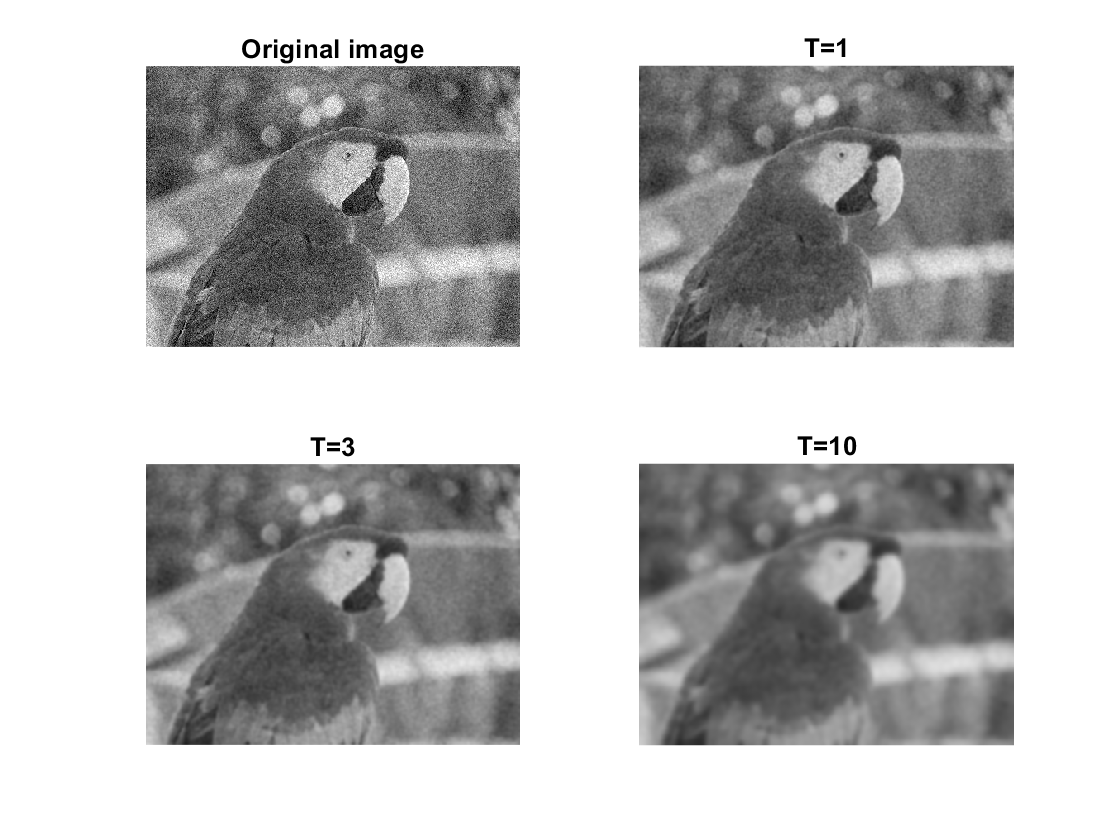
\includegraphics[scale=0.27, trim = 0 12.3cm 1.9cm 1.9cm, clip]{Pictures/Risultati/eq del calore.png}
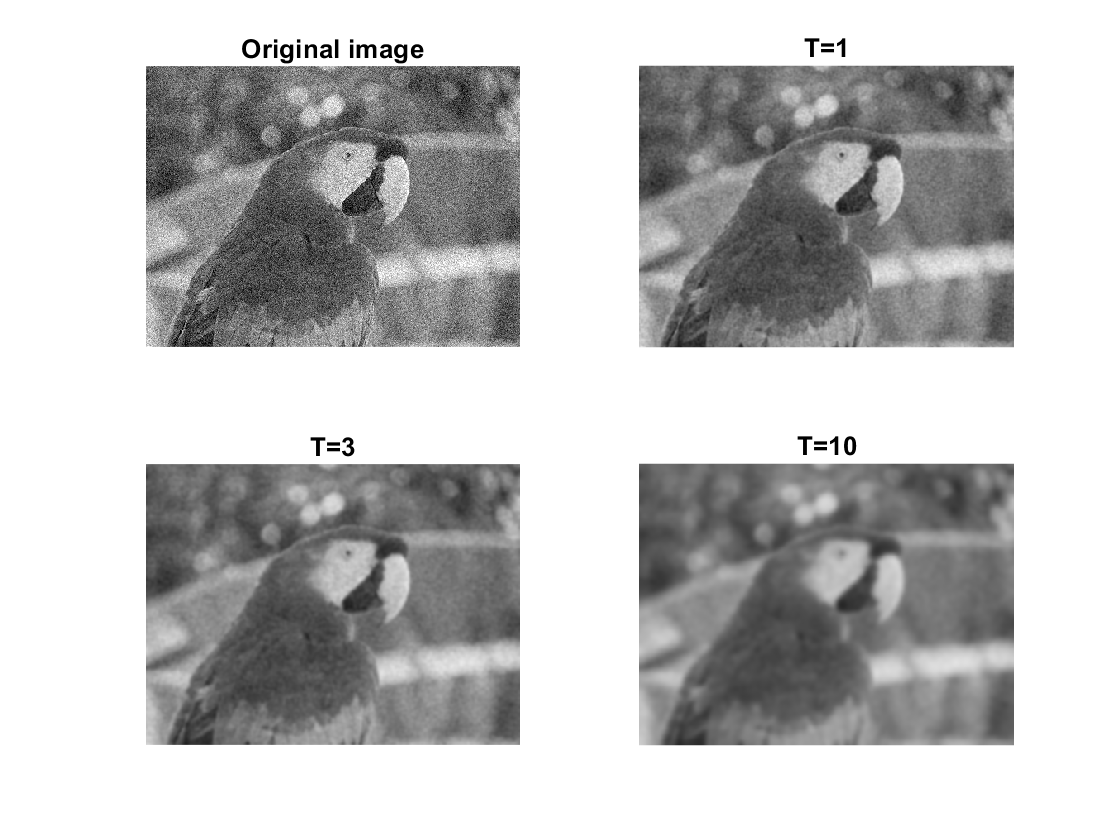
\includegraphics[scale=0.27, trim = 1.9cm 1.7cm 1.9cm 10.3cm, clip]{Pictures/Risultati/eq del calore.png}
\caption{Effetti dell'equazione del calore nel tempo.}\label{fig:figura}
\end{figure}


Questo metodo però non è poi molto utile in generale, sì, il rumore viene eliminato o almeno ridotto ma si perdono importanti dettagli, esistono procedimenti come il metodo Perona-Malik che sono decisamente più utili.\\
L'idea del metodo Perona-Malik è di applicare l'equazione del calore nelle regioni in cui il colore è più uniforme, così da preservarne i bordi.



\section{Rilevamento dei bordi}

Operando una derivata in una data direzione, per il significato in sè di derivata, questa assume valori più elevati quando la variazione è elevata, e assume valori nulli quando non c'è variazione in quella direzione. Per questo motivo, applicata ad un' immagine, ne rileviamo i bordi!\\
Presa una tinta unita la derivata sarà quindi nulla in ogni suo punto (è intuitivo: se un'immagine è una funzione che, date due coordinate restituisce un colore, allora una tinta unita è una funzione costante ed in quanto tale ha derivata nulla).\\
\vspace{1em}
Operando una derivata seconda in una data direzione, per il significato in sè di derivata seconda, questa assume valori più elevati quando la concavità è più stretta, e assume valori pressocchè nulli quando non ci sono concavità (si può pensare alle concavità come a dei picchi o dei ventri, su di una immagine vuol dire chiazze di colore diverso).\\
Presa una sfumatura di colore che varia in maniera lineare, la derivata seconda sarà nulla in ogni suo punto, la derivata prima sarà invece costante. 
\newpage
Si riporta un piccolo script MATLAB che mette in evidenza questo aspetto.
\vspace{1em}
\begin{lstlisting}[language=MATLAB]
%---Operazioni preliminari
Im=imread("nome_immagine.png");	%Apro l'immmagine

[ny, nx, ~]=size(Im)        %Memorizzo le dimensioni dell'immagine
u=double(Im);               %Copia dell'immagine originale su cui lavorare
h=80;                       %Definisco un parametro che usero' per                               enfatizzare i bordi in fase di stampa 


%---Calcolo tutte le derivate
u_x =  u(:,[1 1:nx-1],:) - u;                       %derivata                                                            prima lungo x
u_xx = u(:,[2:nx nx],:) - 2*u + u(:,[1 1:nx-1],:);  %derivata                                                            seconda lungo x
u_y =  u([1 1:ny-1],:,:) - u;                       %derivata                                                            prima lungo y
u_yy = u([2:ny ny],:,:) - 2*u + u([1 1:ny-1],:,:);  %derivata                                                            seconda lungo y
u_xy = u_x([1 1:ny-1],:,:) - u_x;                   %derivata                                                            seconda mista
   
%---Stampo i risultati
figure()
subplot(2,3,2),text(0.3,0,nome,'FontSize',20); axis off
subplot(2,3,4), imshow(Im)
title('Immagine originale')
subplot(2,3,5), imshow(uint8(h*abs(u_x)))
title('h*u_x')
subplot(2,3,6), imshow(uint8(h*abs(u_y)))
title('h*u_y')

figure()
subplot(2,3,2),text(0.3,0,nome,'FontSize',20); axis off
subplot(2,3,4), imshow(Im)
title('Immagine originale')
subplot(2,3,5), imshow(uint8(h*abs(u_x + u_y)))
title('h*(u_x + u_y)')
subplot(2,3,6), imshow(uint8(h*abs(u_xx + u_yy)))
title('h*(u_xx + u_yy)')
\end{lstlisting}

\vspace{1em}
Lo script permette di osservare come con diverse immagini molto semplici se otteniamo i risultati attesi.\\
%\vspace{1em}
\newpage
\begin{figure}[htb] 
\centering
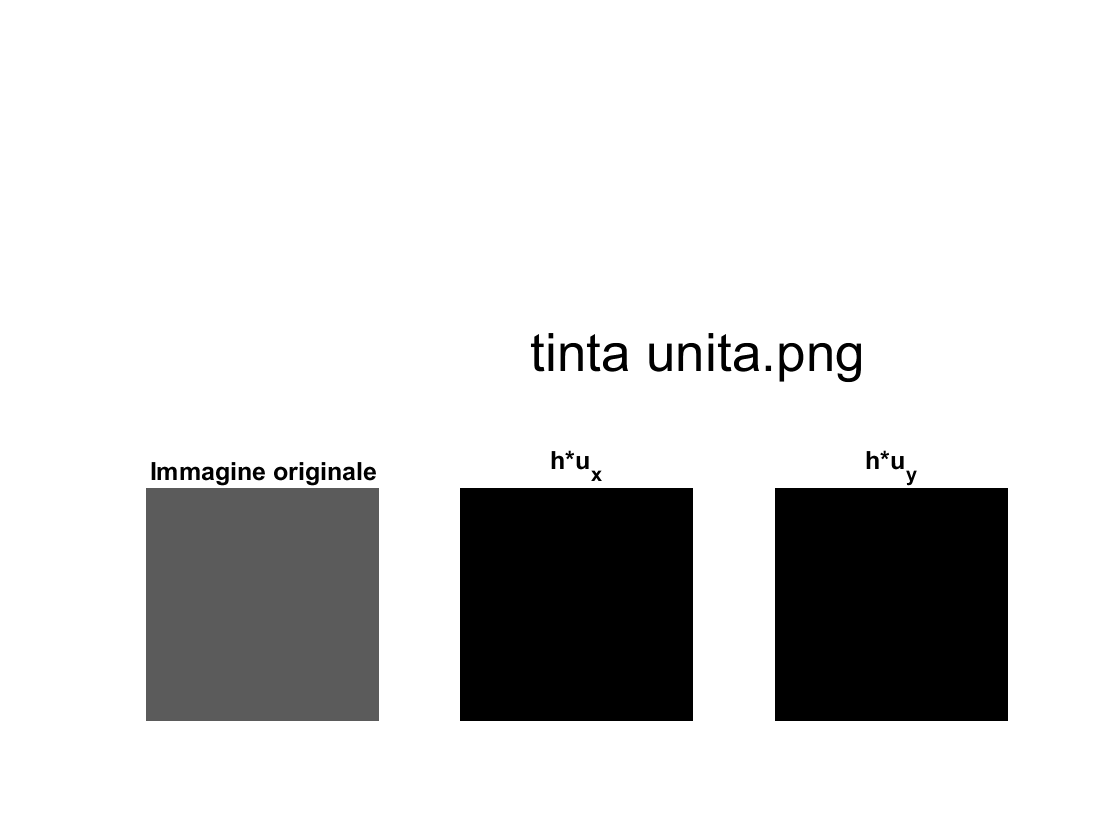
\includegraphics[scale=0.4, trim = 0 0 0 10.5cm, clip]{Pictures/Risultati/tinta unita bianco e nero derivate parziali.png}
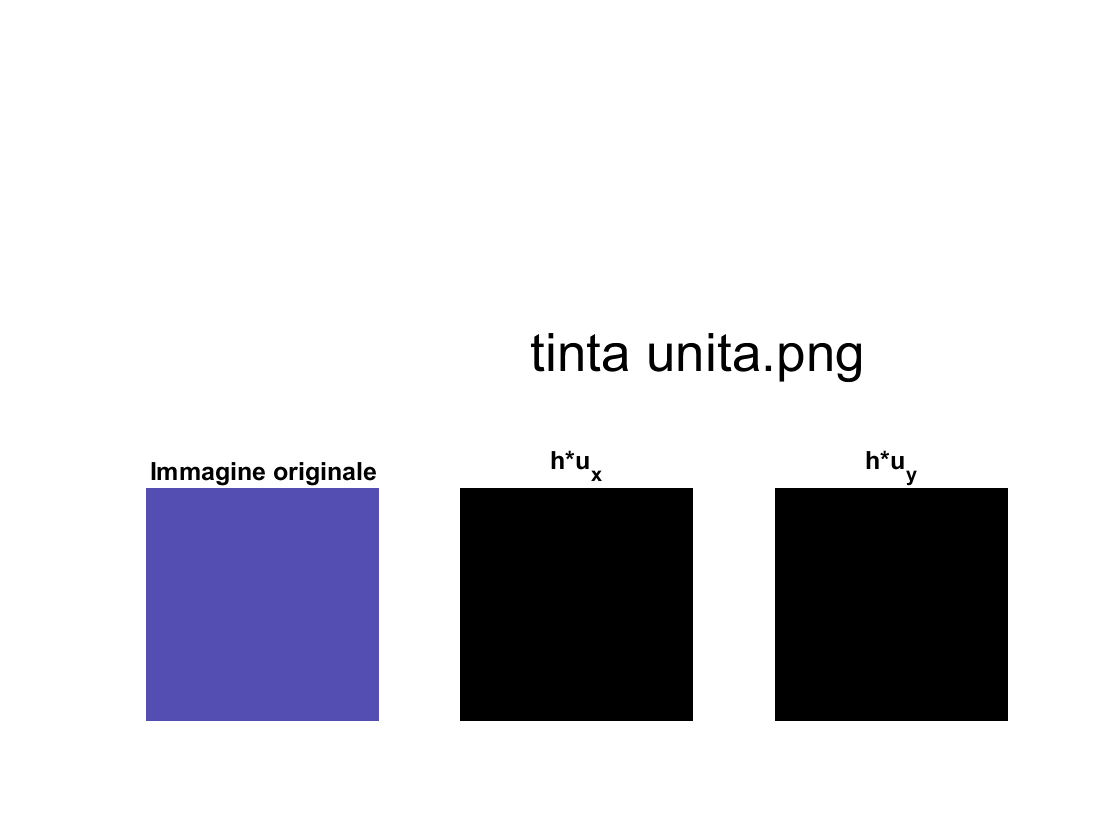
\includegraphics[scale=0.4, trim = 0 0 0 10.5cm, clip]{Pictures/Risultati/tinta unita derivate parziali.png}
\caption{Derivate parziali di una tinta unita.}\label{fig:figura}
\end{figure}

Si può vedere come con un'immagine a tinta unita (che sia essa in bianco e nero o a colori) le derivate sono nulle, quindi lo saranno anche gradiente e laplaciano. Confermiamo inoltre che questi principi valgono sia a colori che in bianco e nero.\\

\newpage
\begin{figure}[htb] 
\centering
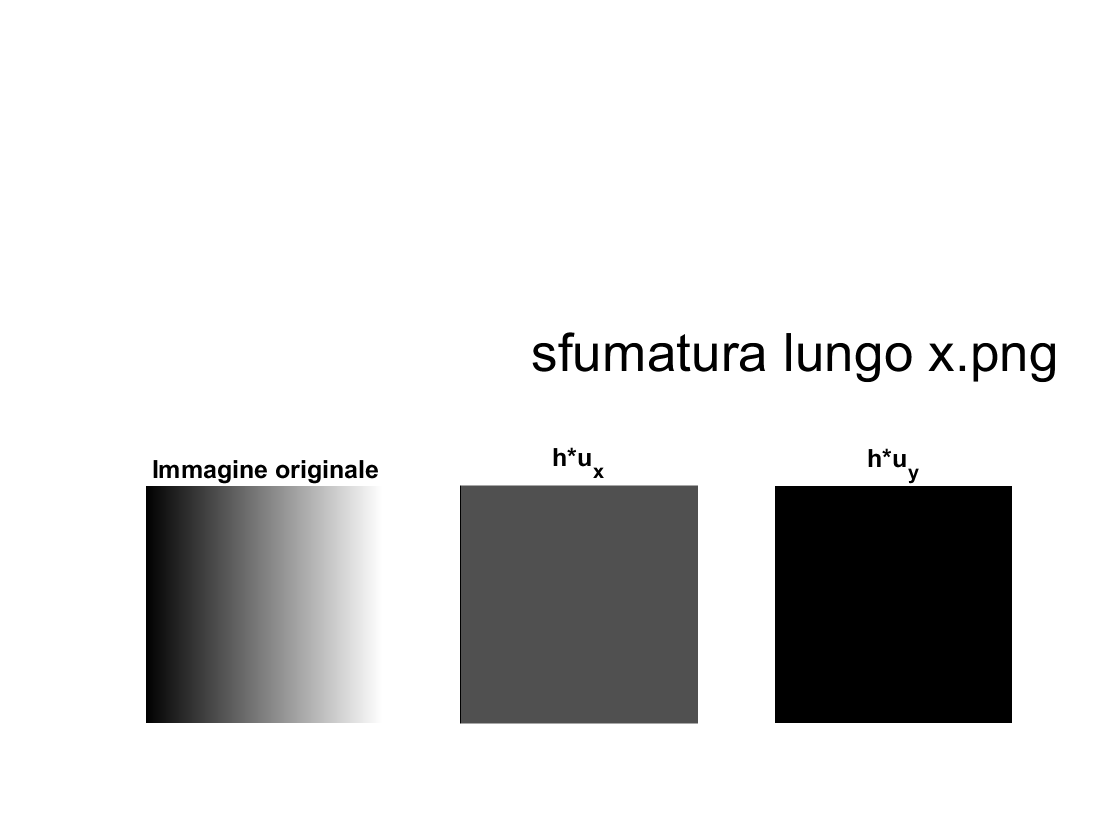
\includegraphics[scale=0.4, trim = 0 0 0 10.5cm, clip]{Pictures/Risultati/sfumatura lungo x bianco e nero derivate parziali.png}
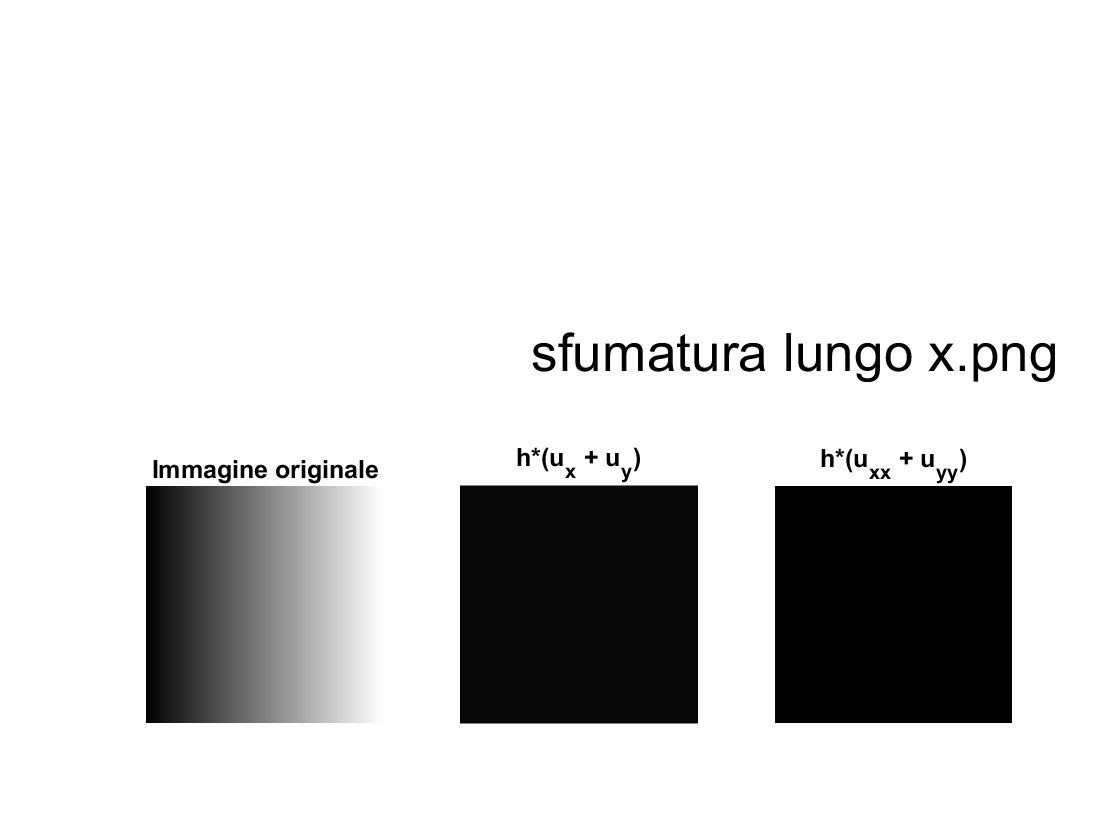
\includegraphics[scale=0.4, trim = 0 0 0 10.5cm, clip]{Pictures/Risultati/sfumatura lungo x bianco e nero gradiente e laplaciano.png}
\caption{Derivate parziali, gradiente e laplaciano di una sfumatura orizzontale.}\label{fig:figura}
\end{figure}

Guardando invece ad una immagine che presenta una sfumatura lineare lungo l'asse x, la derivata lungo x assume un valore costante mentre la derivata lungo y è nulla, proprio perchè lungo y non c'è variazione mentre lungo x c'è una variazione costante.\\
Ovviamente, date queste premesse, il gradiente sarà costante uguale ad $u_x$ (siccome $u_y=0$) e quindi il laplaciano sarà nullo.
Il fatto che in entrambi questi esempi il laplaciano sia nullo è un buon segno, lo useremo per rilevare i bordi ed in queste immagini non ve ne sono, quindi è giusto che il laplaciano sia nullo.\\

\newpage
\begin{figure}   
\centering
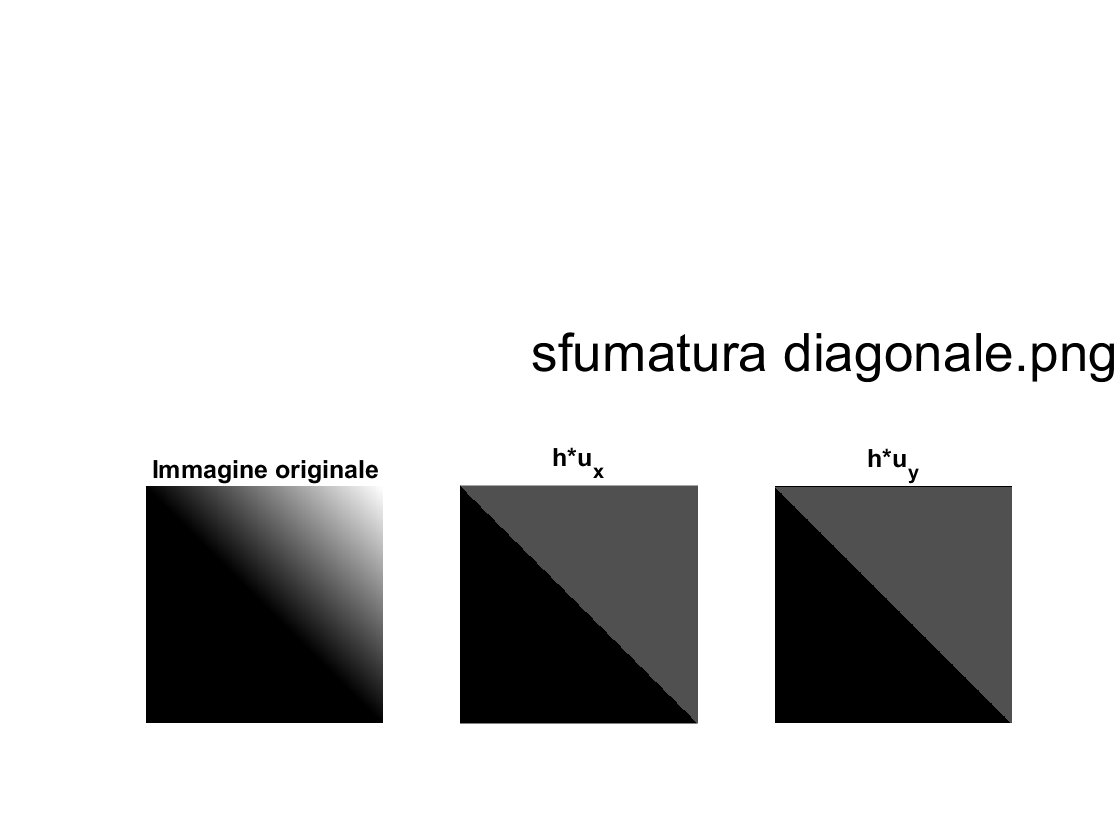
\includegraphics[scale=0.4, trim = 0 0 0 10.5cm, clip]{Pictures/Risultati/sfumatura diagonale bianco e nero derivate parziali.png}
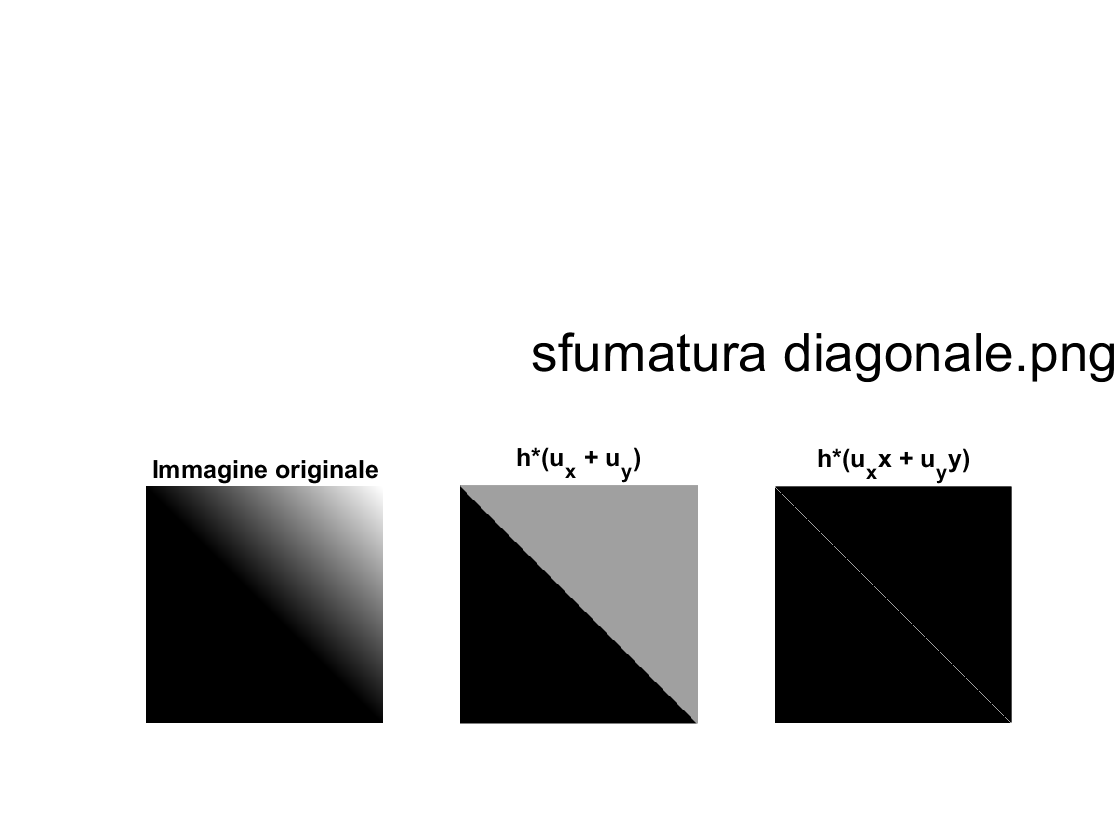
\includegraphics[scale=0.4, trim = 0 0 0 10.5cm, clip]{Pictures/Risultati/sfumatura diagonale bianco e nero gradiente e laplaciano.png}
\caption{Derivate parziali, gradiente e laplaciano di una sfumatura diagonale.}\label{fig:figura}
\end{figure}

Presa una sfumatura diagonale, ma solo su metà immagine vediamo dei riultati interessanti: entrambe le derivate parziali sono nulle nelle regioni in cui non c'è sfumatura, esattamente come nel caso della tinta unita, ed entrambe sono costanti dove c'è sfumatura (che ricordiamo essere lineare).\\
Tutto ciò riconferma quanto visto dai punti precedenti, volgendo quindi uno sguardo al gradiente ed al laplaciano si può notare che mentre il gradiente ha un aspetto molto simile alle due derivate parziali, sommando i loro valori è semplicemente più luminoso, per quanto riguarda il lplaciano la storia cambia. Le derivate seconde sono indicatrici della variazione delle derivate prime, cioè della variazione della variazione del valore della funzione, ma l'unica variazione che hanno le derivate prime è lungo la diagonale.
Abbiamo così individuato il nostro primo bordo, cioè la diagonale che divide di fatto due regioni, una in cui il colore è costante ed una in cui sfuma.\\

\vspace{1em}

Si riporta un ultimo esempio, provando ad introdurre una semplice figura e osserviamo cosa accade.\\

\newpage
\begin{figure}[htb] 
\centering
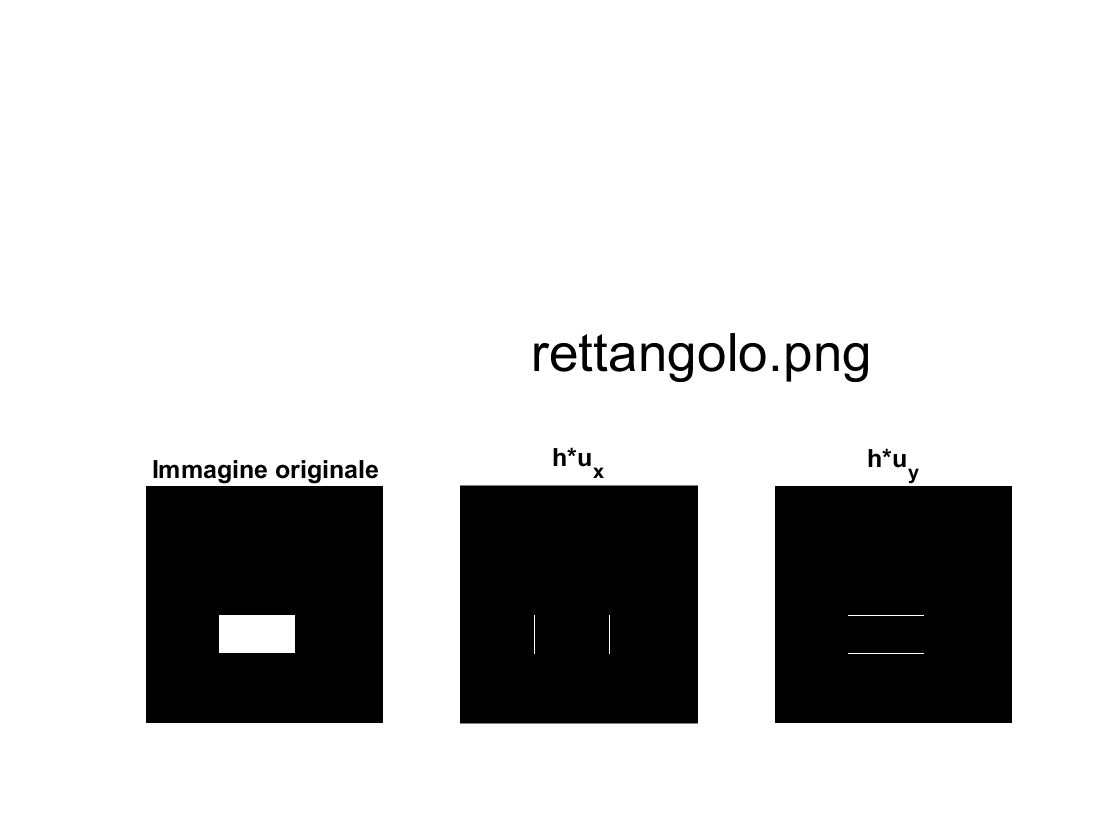
\includegraphics[scale=0.4, trim = 0 0 0 10.5cm, clip]{Pictures/Risultati/rettangolo bianco e nero derivate parziali.png}
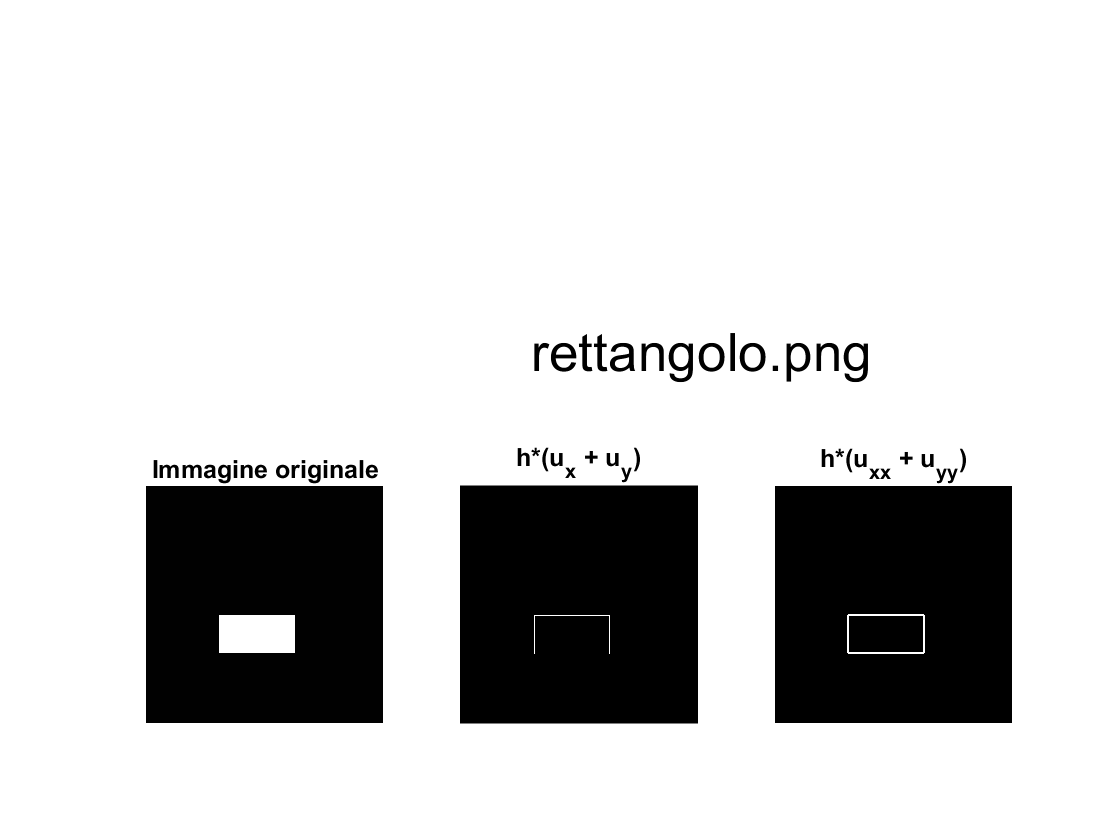
\includegraphics[scale=0.4, trim = 0 0 0 10.5cm, clip]{Pictures/Risultati/rettangolo bianco e nero gradiente e laplaciano.png}
\caption{Derivate parziali, gradiente e laplaciano di una figura semplice.}\label{fig:figura}
\end{figure}

Importando un rettangolo nero su di uno sfondo bianco, come confermato anche dalla prima sfumatura, la derivata lungo x rileva i bordi verticali, quella lungo y i bordi orizzontali, dalla loro somma (quindi dal gradiente) otteniamo già il bordo del rettangolo.
Il bordo così ottenuto è un bordo che idealmente rimarrà inalterato a prescindere dall'ordine della derivata, in particolare quindi anche per derivate seconde, quindi il laplaciano continua a soddisfare la richiesta di determinare i bordi. \\
Come detto: "Il bordo così ottenuto è un bordo che idealmente rimarrà inalterato a prescindere dall'ordine della derivata" è interessante capire perchè. Presa una striscia di pixel, cioè uno strato dell'immagine (la si può immaginare quindi come una funzione da R in R), risulterà essa raffigurare una funzione porta!\\
La funzione porta non è derivabile in senso classico, ripensando alla definizione di derivata avremmo un valore di +infinito prima e -infinito poi. La sua derivata sarà quindi una coppia di delta di Dirac.\\

